\section{Conclusion}
\label{conclusion}

We described an efficient parallel algorithm to compute the number of isomorphic
embeddings of a subgraph in very large networks using MapReduce and the color
coding technique.  We first developed \sahad{} -- a Hadoop based implementation.
We give performance analysis in terms of work and time complexity. We further
explore two approaches to reduce the sorting and communication cost. We also
implement our algorithm using the Harp framework which employs collective
communication and shared memory to facilitates the computation. Our experiments
show that \harpsahad{} has significantly improved performance when compared to
\sahad{} ---  by almost an order of magnitude and simultaneously achieves good
scalability. The new algorithm can process networks with 0.5 Billion edges and 7
node templates. As directions for future research, it would be interesting to
device new algorithms that scale to larger instances. Additionally, it would be
interesting to implement variant of these algorithms for restricted classes of
networks.

\bibliographystyle{abbrv}
\bibliography{zz}

% biography section
% 
% If you have an EPS/PDF photo (graphicx package needed) extra braces are
% needed around the contents of the optional argument to biography to prevent
% the LaTeX parser from getting confused when it sees the complicated
% \includegraphics command within an optional argument. (You could create
% your own custom macro containing the \includegraphics command to make things
% simpler here.)
%\begin{IEEEbiography}[{\includegraphics[width=0.8in,height=1in,clip,keepaspectratio]{mshell}}]{Michael Shell}
% or if you just want to reserve a space for a photo:

\vspace{-1.5cm}

\begin{IEEEbiography}[{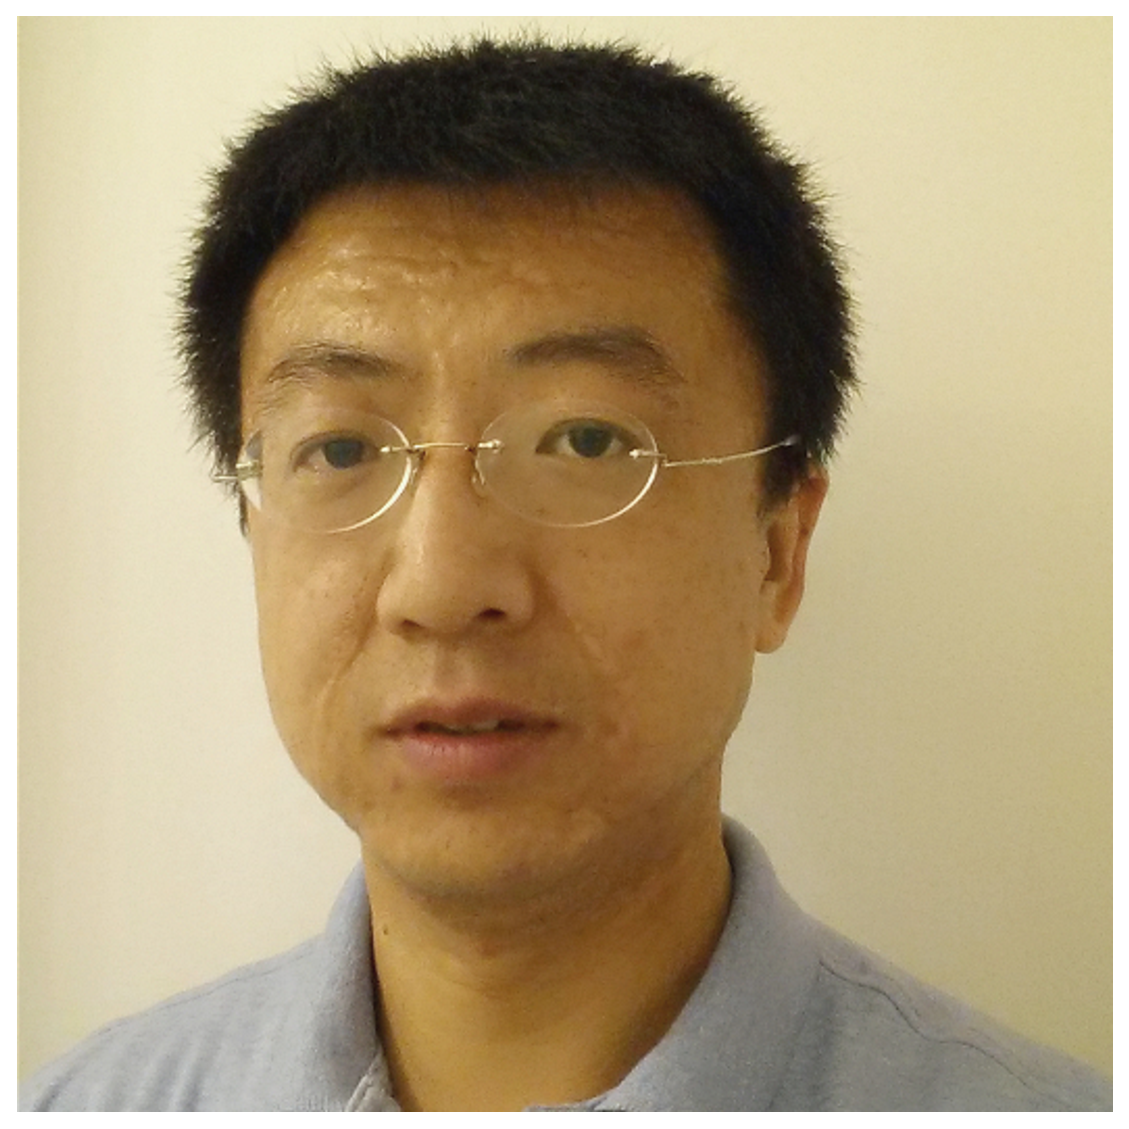
\includegraphics[width=0.75in,clip,keepaspectratio]{authors-pic/zhaozhao-new.eps}}]{Zhao Zhao}
is pursuing his Ph.D degree  in Computer Science at Virginia Tech. He is also  a
Software Engineer in Verisign Labs, Verisign Inc. His research interests are in
Network Science and analytics, especially in the design and analysis of parallel
graph algorithms.  \end{IEEEbiography}

\vspace{-2.5cm}

\begin{IEEEbiography}[{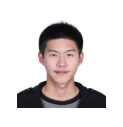
\includegraphics[width=0.8in,clip,keepaspectratio]{authors-pic/limeng-new.eps}}]{Meng Li}
 is a Computer Science Ph.D. student in the School of informatics and Computing
 at Indiana University. His advisor is Prof. Judy Qiu. His research interest is
 distributed systems and parallel computing.  \end{IEEEbiography}

\vspace{-2.5cm}

\begin{IEEEbiography}[{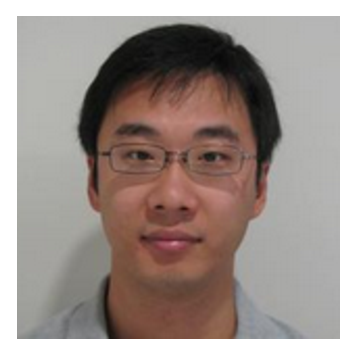
\includegraphics[width=0.8in,clip,keepaspectratio]{authors-pic/guanying.eps}}]{Guanying Wang}
 earned his PhD in Computer Science from Virginia Tech in 2012. He is now a
 software engineer at Google.  \end{IEEEbiography}

\vspace{-2.5cm}

\begin{IEEEbiography}[{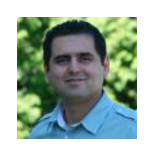
\includegraphics[width=0.8in,clip,keepaspectratio]{authors-pic/ali.eps}}]{Ali Butt}
 received his Ph.D. degree in Electrical \& Computer Engineering from Purdue
 University in 2006. He is a recipient of an NSF CAREER Award, IBM Faculty
 Awards, a VT College of Engineering (COE) Dean's award for "Outstanding New
 Assistant Professor", and NetApp Faculty Fellowships. Ali's research interests
 are in distributed computing systems and I/O systems.  \end{IEEEbiography}

\vspace{-2.0cm}

\begin{IEEEbiography}[{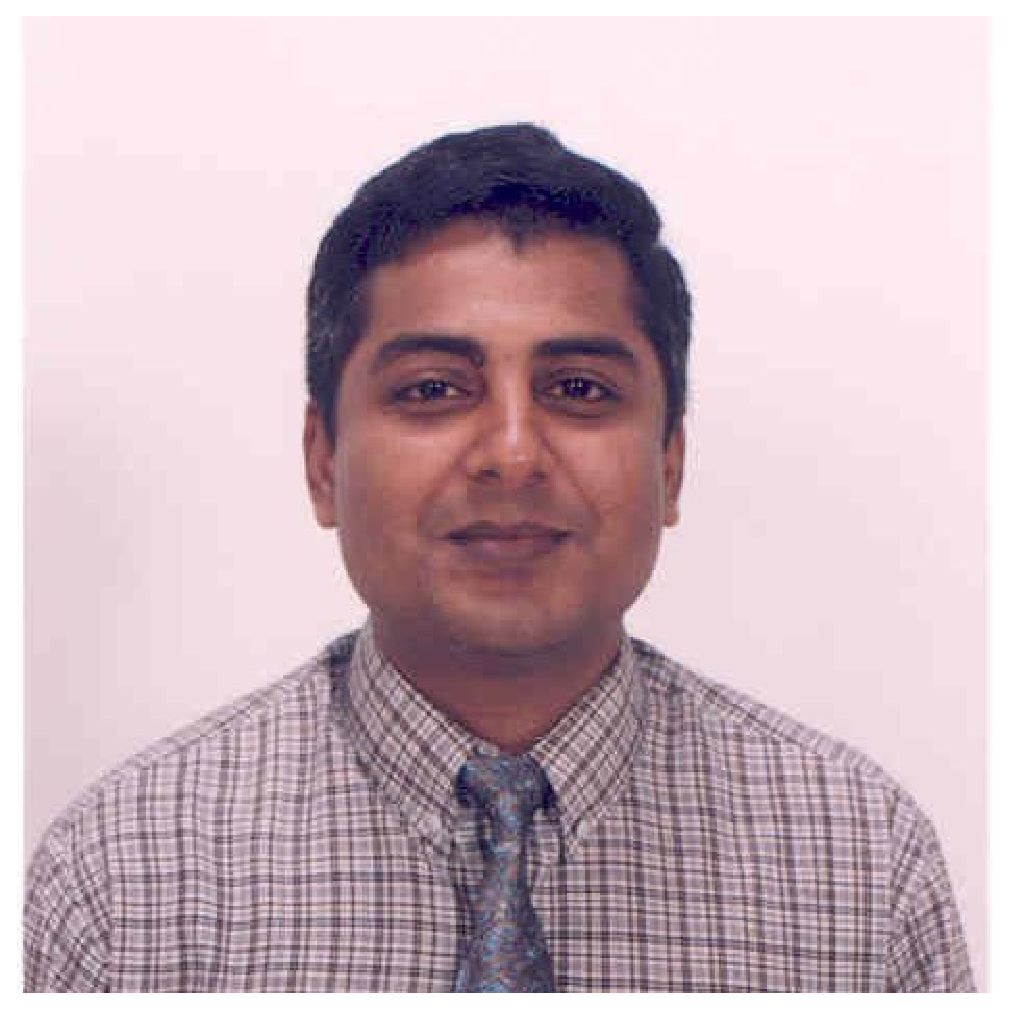
\includegraphics[width=0.8in,clip,keepaspectratio]{authors-pic/maleq-new.eps}}]{Maleq Khan} is an Assistant Professor in the Department of Electrical Engineering and Computer Science at Texas A\&M University--Kingsville. He received his Ph.D. in Computer Science from Purdue University. His research interests are in parallel and distributed computing, big data analytics, high performance computing, and data mining. 
 \end{IEEEbiography}

\vspace{-2.2cm}

\begin{IEEEbiography}[{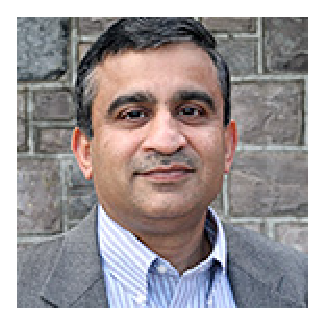
\includegraphics[width=0.8in,clip,keepaspectratio]{authors-pic/madhav.eps}}]{Madhav Marathe}
 is a professor of Computer Science and the Director of  the Network
 Dynamics and Simulation Science Laboratory, Biocomplexity Institute, Virginia Tech.
 His research interests include high performance computing, modeling and simulation, theoretical computer science
 and socio-technical systems. He is a fellow of the IEEE, ACM and AAAS.
\end{IEEEbiography}

\vspace{-2.2cm}

\begin{IEEEbiography}[{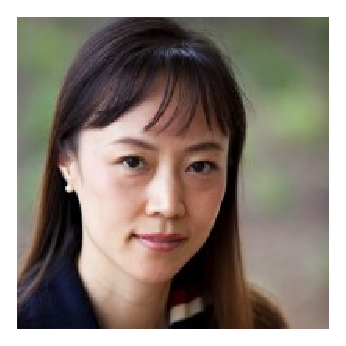
\includegraphics[width=0.8in,clip,keepaspectratio]{authors-pic/judy.eps}}]{Judy Qiu}
 is an associate professor of Intelligent Systems Engineering in the School of
 Informatics and Computing at Indiana University. Her research interests are
 parallel and distributed systems, cloud computing, and high-performance
 computing. Her research has been funded by NSF, NIH, Intel, Microsoft, Google,
 and Indiana University. Judy Qiu leads the Intel Parallel Computing Center
 (IPCC) site at IU. She is the recipient of a NSF CAREER Award in 2012.
 \end{IEEEbiography} 
 
\vspace{-1.8cm}

\begin{IEEEbiography}[{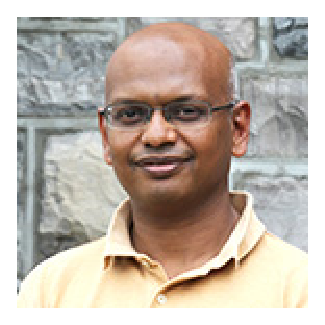
\includegraphics[width=0.8in,clip,keepaspectratio]{authors-pic/anil.eps}}]{Anil Vullikanti}
 is an Associate Professor in the Department of Computer Science and the 
  Biocomplexity Institute of Virginia
 Tech. His interests are in the areas of approximation and randomized algorithms, 
distributed computing, graph dynamical systems and their applications to
epidemiology, social networks and wireless networks.  He is a
 recipient of the NSF and DOE Career awards.  \end{IEEEbiography}

% if you will not have a photo at all:
%\begin{IEEEbiographynophoto}{John Doe}
%Biography text here.
%\end{IEEEbiographynophoto}

% insert where needed to balance the two columns on the last page with
% biographies
%\newpage

% You can push biographies down or up by placing
% a \vfill before or after them. The appropriate
% use of \vfill depends on what kind of text is
% on the last page and whether or not the columns
% are being equalized.

%\vfill

% Can be used to pull up biographies so that the bottom of the last one
% is flush with the other column.
%\enlargethispage{-5in}



% that's all folks
\end{document}


